\documentclass[border=10pt]{standalone}

\usepackage{tikz}
\usepackage{tikzsymbols}
\usetikzlibrary{calc,patterns,shapes.geometric}

\def\centerarc[#1](#2)(#3:#4:#5){\draw[#1] ($(#2)+({#5*cos(#3)},{#5*sin(#3)})$) arc (#3:#4:#5);}

\begin{document}
	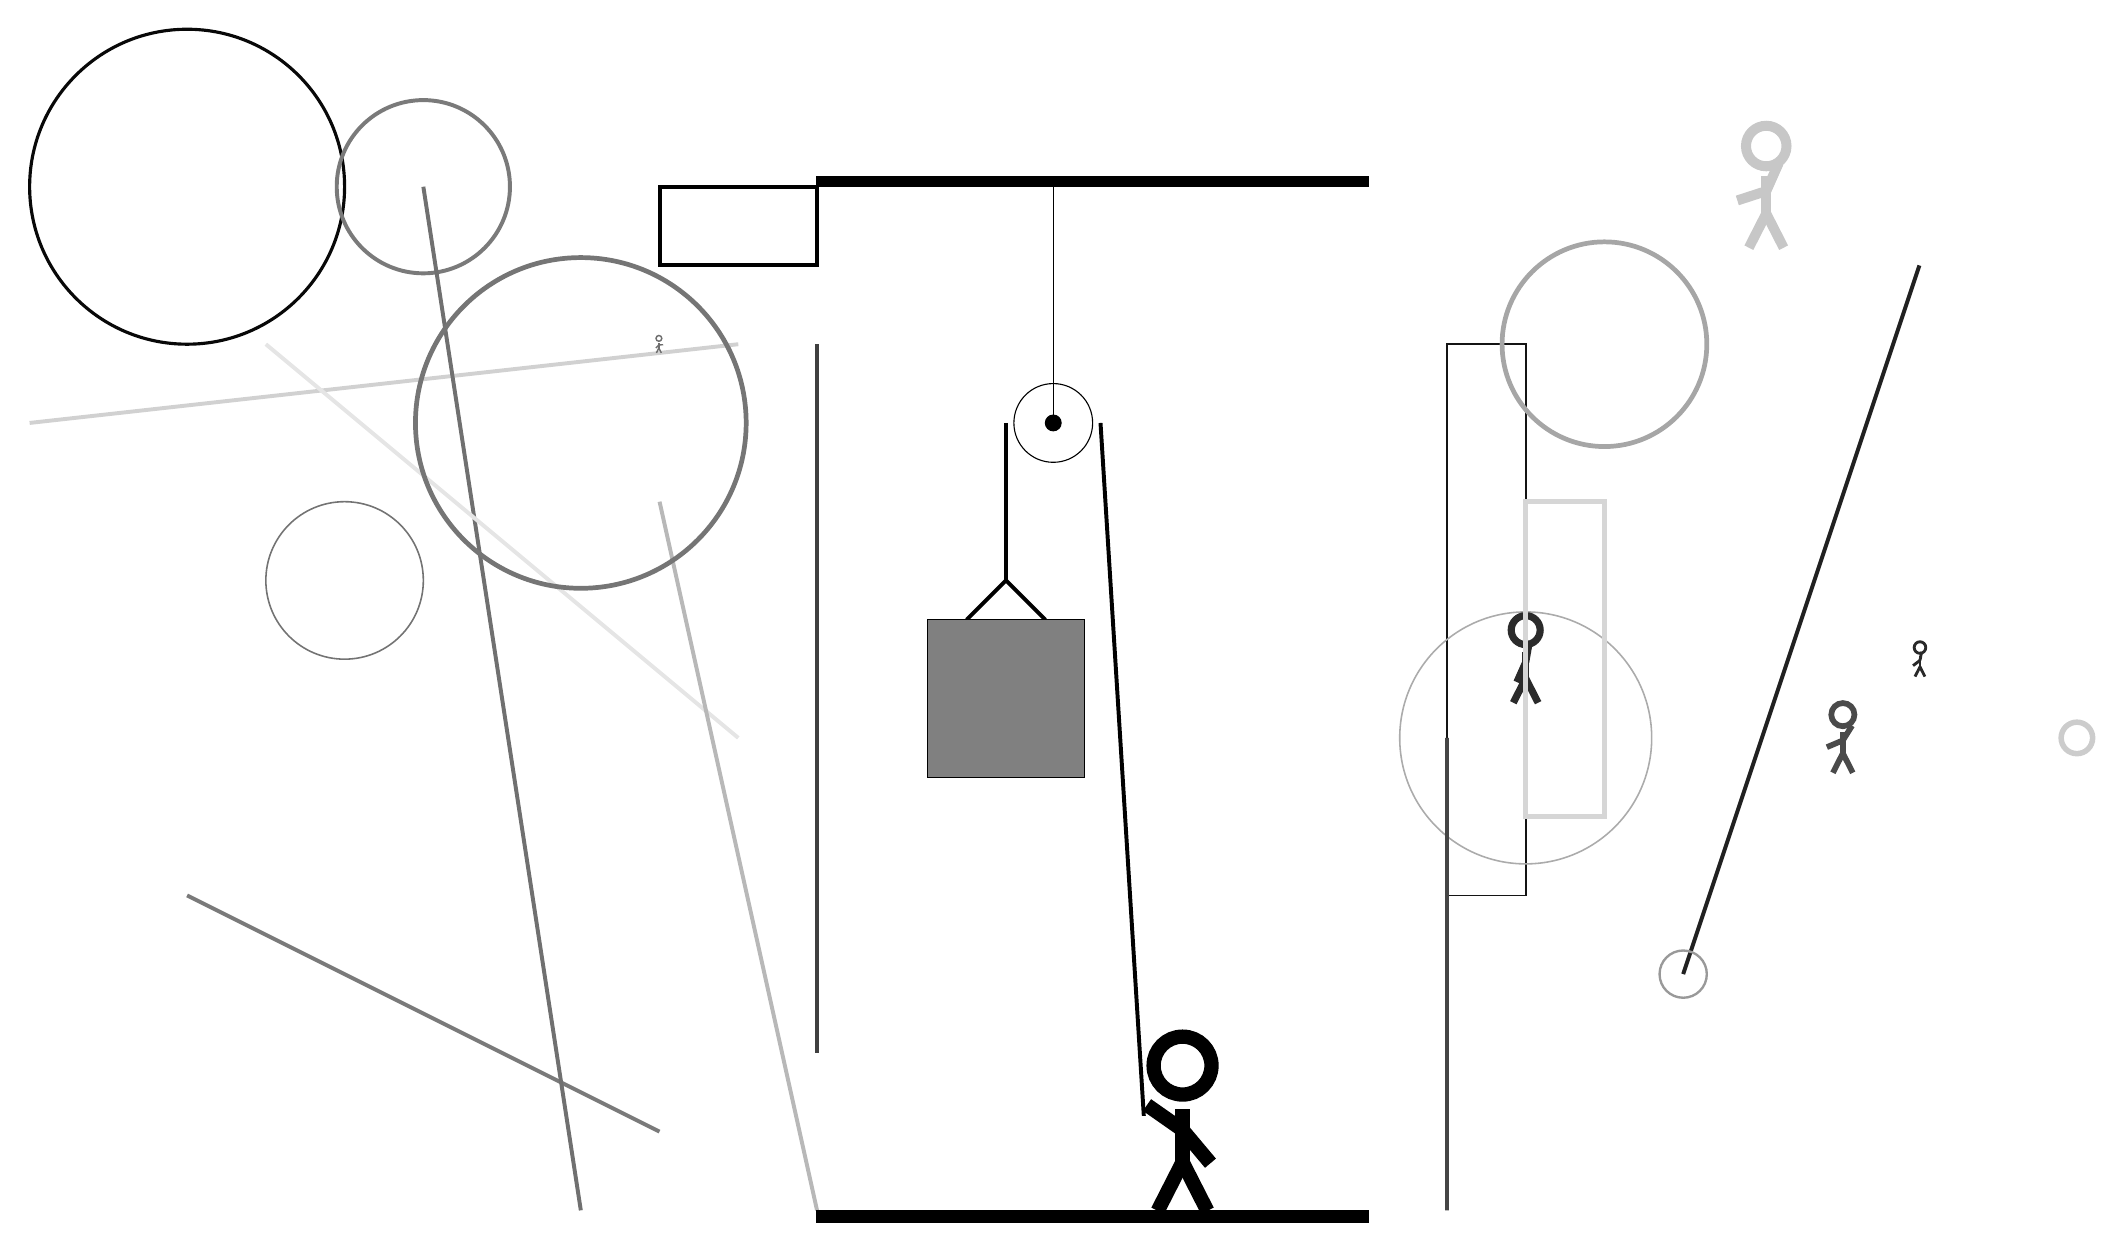
\begin{tikzpicture}
		%%%%% START %%%%%
		
		\draw[fill=black] (-2, 10) rectangle (5, 10.125);
		
		\draw (1, 7) circle (0.5);
		\draw[fill=black] (1, 7) circle (0.1);
		\draw (1, 10) -- (1, 7);
		
		\draw[line width=0.5mm] (-0.1, 4.5) -- (0.4, 5.0) -- (0.9, 4.5);
		\draw[fill=black!50] (-0.6, 4.5) rectangle (1.4, 2.5);
		
		\draw[line width=0.5mm, color=black!18](-3, 8) -- (-12, 7);
		
		\node[line width=0.2mm, color=black!71] at (11, 3) {\Strichmaxerl[4][23][58]};
		\draw[line width=0.6mm, color=black!75] (-2, 8) rectangle (-2, -1);
		\node[line width=0.6mm, color=black!84] at (12, 4) {\Strichmaxerl[2][37][79]};
		\draw [line width=0.7mm, color=black!20](14, 3) circle (0.2);
		
		\draw[line width=0.5mm, color=black!87](9, 0) -- (12, 9);
		\draw[line width=0.2mm, color=black!92] (6, 1) rectangle (7, 8);
		\node[line width=0.6mm, color=black!57] at (-4, 8) {\Strichmaxerl[1][46][1]};
		\draw [line width=0.2mm, color=black!33](7, 3) circle (1.6);
		
		\draw [line width=0.2mm, color=black!55](-8, 5) circle (1.0);
		\draw[line width=0.5mm, color=black!52](-4, -2) -- (-10, 1);
		\draw[line width=0.5mm, color=black!100] (-2, 10) rectangle (-4, 9);
		\draw [line width=0.4mm, color=black!97](-10, 10) circle (2.0);
		
		\draw [line width=0.6mm, color=black!35](8, 8) circle (1.3);
		\node[line width=0.5mm, color=black!83] at (7, 4) {\Strichmaxerl[5][66][80]};
		\draw [line width=0.5mm, color=black!52](-7, 10) circle (1.1);
		
		\node[line width=0.6mm, color=black!22] at (10, 10) {\Strichmaxerl[7][18][66]};
		
		\draw [line width=0.3mm, color=black!40](9, 0) circle (0.3);
		\draw[line width=0.5mm, color=black!56](-5, -3) -- (-7, 10);
		\draw[line width=0.5mm, color=black!10](-3, 3) -- (-9, 8);
		\draw[line width=0.5mm, color=black!28](-4, 6) -- (-2, -3);
		\draw[line width=0.4mm, color=black!73] (6, 3) rectangle (6, -3);
		\draw[line width=0.7mm, color=black!16] (7, 2) rectangle (8, 6);
		\draw [line width=0.6mm, color=black!54](-5, 7) circle (2.1);
		
		\draw[line width=0.5mm] (0.4, 7) -- (0.4, 5.0);
		\centerarc[line width=0.5mm](1, 7)(0:180:0.6);
		\draw[line width=0.5mm](1.6, 7) -- (2.15, -1.8);
		
		\node at (2.6, -1.9) {\Strichmaxerl[10][-35][-50]};
		
		\draw[fill=black] (-2, -3) rectangle (5, -3.15);
		
		%%%%% END %%%%%
	\end{tikzpicture}
\end{document}